\chapter{自发运动:运动皮层} \label{chap:chap34}
在本章中,我们将描述大脑皮层如何使用来自外部世界的感觉信息来指导运动动作,从而使个体能够与周围环境互动。 我们首先对随意运动一词的含义进行一般描述,并介绍一些理解其控制的理论框架,然后是涉及随意运动行为的皮层回路的基本解剖结构。 然后我们考虑与身体、外部空间和行为目标相关的信息如何在顶叶皮层区域组合和处理。 随后讨论运动前皮层区域在选择和规划运动动作中的作用。 最后,我们检查了初级运动皮层在运动执行中所起的作用。

\section{自主运动是行动意图的身体表现}
包括人类在内的动物拥有神经系统,不仅是为了感知世界或思考世界,而且主要是为了与之互动以生存和繁殖。 了解有目的的行为是如何实现的是神经科学的巨大挑战之一。 我们在此关注大脑皮层对随意运动行为的控制,特别是灵长类动物的随意手臂和手部运动。

与由传入的感官刺激自动触发的刻板固定延迟反射反应(第 32 章)相反,自主运动是有目的的、有意的和依赖于上下文的,并且通常伴随着(至少在人类中)一种“主人翁感” ”的行为,感觉这些行为是由个人故意造成的。 采取行动的决定通常是在没有外部触发刺激的情况下做出的。 此外,世界上不断变化的事件和条件提供了不断变化的行动机会,因此自愿行动涉及备选方案之间的选择,包括选择不采取行动。 最后,根据当前上下文,同一对象或事件可以在不同时间引发不同的动作。

在整个进化过程中,自愿行为的这些特征在高等灵长类动物中变得越来越突出,尤其是在人类中,这表明控制灵长类动物自愿行为的神经回路具有适应性。 特别是,进化导致感官输入的物理特性与其对个体的行为显着性的分离程度越来越大。 控制电路的适应还通过允许个人记住和从以前的经验中学习,预测不同行动选择的未来结果,并采用新策略和找到新的解决方案来实现他们的目标,从而增强了一个物种可用的自愿运动行为 期望的目标。 自主控制如何、何时甚至是否行动,赋予灵长类动物自主行为以丰富性和灵活性,并防止行为变得冲动、强迫甚至有害。

自愿行为是个人对环境采取行动的意图的物理表现,通常是立即或在未来某个时候实现目标。 这可能需要针对当前条件和个人的长期目标量身定制的单一非刻板动作或动作序列。 独立于运动而使用手指、手和手臂的能力进一步帮助灵长类动物,尤其是人类,利用他们的环境。 大多数动物在饥饿时必须在周围环境中寻找食物。 相比之下,人类可以通过用手做饭来“觅食”,或者只需在手机上输入几个数字就可以订购外卖食物。 由于大脑皮层的大面积涉及自主运动控制的各个方面,因此对自主运动的皮层控制的研究为了解整个大脑皮层的目的性功能组织提供了重要的见解。


\subsection{理论框架有助于解释行为和自愿控制的神经基础}
个人获取环境信息和身体与环境的关系、决定如何与环境互动以实现短期或长期目标、组织和执行自愿运动以实现目标的神经过程 他们的目标传统上分为三个分析组成部分:感知机制生成外部世界和其中个体的内部表征,认知过程使用这个世界的内部模型来选择与环境交互的行动过程,以及所选择的 然后将行动计划传递给电机系统以供实施。 这种大脑整体功能组织的连续观点长期以来一直主导着神经科学。 例如,这本教科书有单独的部分专门介绍感知、认知和运动。

大脑必须将目标转化为实现目标的运动命令。 例如,喝一口咖啡需要大脑将有关咖啡杯的视觉信息和有关您手臂和手的当前姿势和运动的躯体信息转换为一种肌肉收缩模式,使您的手移向杯子,抓住它, 然后将它举到嘴边。 许多行为和建模研究表明,这可以通过一系列感觉运动坐标转换来实现,这些转换将视杯的视网膜图像转换为运动命令(图 34-1A)。

这种感觉运动转换模型的变体指导了许多关于自主手臂运动控制的研究的设计和解释。 神经记录研究,包括许多将在此处描述的研究,已经发现运动参数和感觉运动转换的可能神经相关性,这些运动被认为是运动计划和执行的基础。 这个概念框架是大脑功能的代表性模型的一个例子。 正如初级感觉区域神经元的活动似乎编码刺激的特定物理特性一样,感觉运动转换模型假设运动系统中神经元的活动明确编码或表示预期运动的特定特性和参数。

然而,感觉运动转换模型有重要的局限性。 其中,此类模型中通常使用的参数和坐标系是从物理学和工程学中引入的,而不是从生物传感器和效应器的生理特性中推导出来的。 此外,该模型将所有重点都放在严格的串行前馈计算上,并将反馈电路主要用于检测和纠正性能错误。 该模型还要求在电机系统生成任何电机命令之前明确计算运动的每个时间细节。 另一个限制是它的刚性; 它假设相同的计算序列控制着每个上下文中的每个动作。 最后,这种方法没有解决所提出的感觉运动转换如何由神经元实现的问题。

近年来,电机系统的理论研究已经从严格的表征模型转向更动态的因果模型。 这种方法的前提是电机控制电路的功能架构进化为产生运动,而不是表示它们的参数。 这些回路特性是通过神经回路的进化变化和出生后发育过程中依赖于经验的适应过程获得的,这些过程在神经回路内产生了产生所需运动所必需的突触连接模式。 脊髓和脊髓上运动回路确保脊髓运动神经元在任务条件下产生适当的肌肉收缩信号,而不依赖于坐标变换等计算形式。

一个这样的理论框架是最优反馈控制(图 34-1B;参见第 30 章)。 有许多不同形式的最优控制,每一种都抓住了控制的重要方面。 最优反馈控制,顾名思义,强调反馈信号对于运动规划和控制的重要性。 从某种意义上说,它是最佳的,因为它强调了行为目标和当前环境在确定如何最好地计划和控制运动方面的重要性。 这种灵活性可以解释人类的运动表现如何既高度可变又成功。

最优反馈控制框架还将自主运动的控制分为三个关键过程:状态估计、任务选择和控制策略(图 34-1B)。 状态估计涉及前向内部模型,这些模型使用运动命令的效应副本和外部感觉反馈来提供对身体和环境当前状态的最佳估计(第 30 章)。 任务选择涉及大脑在当前环境中选择行为目标的神经过程,以及哪些运动动作可能最好地实现该目标。 这种选择可以基于支持替代行动和实现目标的替代选择的感官证据,以及影响最佳反应的其他因素,例如动机状态、任务紧迫性、偏好、相对收益与风险、身体的机械特性 和环境,甚至是不同行动选择的生物力学成本。 最后,控制策略提供了一组规则和计算,用于确定如何生成电机命令以在给定身体和环境的当前状态下实现行为目标。 重要的是,最佳反馈控制中的控制策略过程不是一系列纯前馈计算,用于计算运动开始前所需运动轨迹和相关肌肉活动模式的每个瞬时细节。 相反,它涉及对反馈电路增益进行依赖于上下文和时间的调整,允许肌肉活动的时空形式实时动态出现,作为运动生成的控制过程的一部分。

感觉运动转换和最优反馈控制模型并不是互不相容的假设。 最佳反馈控制解释了运动行为的某些特征,但在很大程度上与控制的神经实现无关。 它假设电机电路是动态系统,可以在不同的任务约束下达到预期的目标。 因此,给定的神经元可能有助于不同任务条件下的感觉运动控制,但其活动可能不对应于可定义坐标框架中的特定运动参数。 相比之下,感觉运动转换模型并没有完全解释实时运动控制是如何通过运动电路实现的,而是强调需要将信息从感觉信号转换为运动指令。

即使神经控制系统是动态的,它控制的系统——肌肉骨骼植物——也是一个物理对象,必须遵守普遍的物理运动定律。 因此,神经活动应该显示出与那些有助于推断这些神经元如何促进自主运动控制的物理参数和规律的相关性,即使它们并不试图对这些术语进行编码。 事实上,分离不同类型的运动相关信息的实验任务揭示了不同皮质运动区域的神经活动如何与不同的运动特性以及运动计划和执行的不同方面相关联的重要差异。 最后,我们可以对我们的移动方式施加任意的意志控制。 例如,我们可以选择沿着一条直线路径高效地进行无障碍的到达运动,或者异想天开地沿着一条复杂的弯曲路径进行运动,即使没有需要避开的障碍,而且运动消耗的能量也很大。 实验挑战是揭示大脑如何通过神经元和神经回路实施这种有意的控制。


\subsection{许多额叶和顶叶皮层区域参与自主控制}
在这里,我们描述了额叶和顶叶皮层的区域,这些区域将感觉输入转化为运动指令以产生自主运动。 然后,我们检查了参与自愿控制手臂和手部运动的神经回路,这些运动是灵长类动物运动库的重要组成部分。 我们专注于恒河猴 (Macaca mulatta) 的研究,因为我们对手臂和手的皮质控制的大部分知识都来自这个物种,而人类自主控制的神经回路似乎具有类似的组织。 许多其他神经结构,包括前额皮质、基底神经节和小脑,也在以目标为导向的自愿行为的整体组织中发挥关键作用(第 37 和 38 章)。

根据细胞结构和骨髓结构细节的区域差异、皮质-皮质连通性、不同标记分子的分布以及神经反应特性的区域差异,已经使用了几种不同的命名法来划分中央前、中央后和顶叶皮层。 在这里,我们将使用一些更广泛接受的术语,而不描述各种命名法之间的近似同源性。

基于 Brodmann 对人类的开创性细胞构造研究,猴子大脑皮层的不同叶被分为更小的区域,包括中央前皮质中的两个(区域 4 和 6),中央后皮质中的四个(区域 1、2、3a、 和 3b),并且在上顶叶皮层和下顶叶皮层中至少有两个(区域 5 和 7)。 虽然这些细胞结构分裂在文献中仍然存在,但随后的解剖学和功能研究已经从根本上改变了人们对中央前皮层和顶叶皮层组织方式的看法(图 34-2)。

目前的地图通常将初级运动皮层 (M1)(灵长类动物中最直接参与运动执行的皮层区域)置于 Brodmann 区 4。Brodmann 区 6 现在通常分为五个或六个功能区,主要涉及大脑的不同方面 身体不同部位运动的规划和控制。 手臂控制区域包括背侧前运动皮层 (PMd) 和前运动前皮层 (pre-PMd),分别位于外侧区域 6 背侧凸面的尾部和喙部。 手部控制区域包括腹侧前运动皮层 (PMv),位于区域 6 的腹侧凸面上,该区域已进一步分为两个或三个较小的子区域。 在内侧前运动皮层区域发现了与运动选择、排序和启动相关的各种功能。 其中包括皮层半球内侧表面的一个区域,该区域最初被 Woolsey 及其同事发现并称为次级运动皮层,但现在被称为辅助运动区。 该区域又分为两个区域,一个位于尾部的辅助运动区(SMA)和一个位于喙部的预辅助运动区(pre-SMA)。 在 Brodmann 区 6 之外,三个额外的运动区域,背侧、腹侧和嘴侧扣带回运动区(分别为 CMAd、CMAV 和 CMAr)也参与运动选择,但尚未像更多的外侧运动前区那样得到充分研究 .

初级体感皮层(S-I;包括区域 1、2、3a 和 3b)位于前中央后回。 它处理来自外围的皮肤和肌肉机械感受器信号,并将该信息传输到其他顶叶和中央前皮层区域(第 19 章)。 与区域 6 一样,Brodmann 的顶叶区域 5 和 7 现在被划分为位于顶叶内沟 (IPS) 内和附近的几个区域,每个区域都集成了关于身体的各种类型的感觉信息或用于自主运动控制的空间目标。 这些包括顶叶区域 PE 和 PEc 在头侧或上侧,以及 PF、PFG、PG 和尾侧、下侧的 OPT。 IPS 内的区域包括前、外侧、内侧和腹侧顶内区域(分别为 AIP、LIP、MIP 和 VIP)以及顶内区域 PEip 和更高的视觉区域 V6A。

这些中央前、中央后和顶叶皮层区域通过相互、会聚和发散投射的复杂模式相互连接。 SMA、PMd 和 PMv 不仅与 M1 之间而且彼此之间也具有体表组织的相互联系。 SMA 和 M1 都接收来自 S-I 和背顶叶皮层的躯体组织输入,而 PMd 和 PMv 与顶叶皮层的尾部、内侧和外侧部分相互连接。 这些体感和顶叶输入为初级运动和尾部运动前区提供与行为目标、目标对象以及用于计划和引导运动行为的身体位置和运动相关的感觉信息。

相比之下,pre-SMA 和 pre-PMd 投射到 SMA 和 PMd 但不投射到 M1,并且与顶叶的连接很弱。 相反,它们与前额叶皮层具有相互联系,因此可能会对自愿行为施加更随意的依赖于上下文的控制。 前额皮质也与其他前运动皮质区域相连。

手和手臂运动的控制是通过分布在几个顶叶和中央前运动区域的部分隔离的并联电路来实现的。 手部运动功能通常由位于更横向的额顶叶回路支持,尤其是 AIP 和 PMv。 相比之下,近端手臂运动功能由更内侧的回路支持,特别是顶叶区域 PE 和 MIP 以及中央前区域 PMd、SMA 和前 SMA。




\subsection{下行运动命令主要由皮质脊髓束传递}
较旧的教科书通常将初级运动皮层 (M1) 称为“最终共同路径”。 其他皮层运动区被认为通过投射到 M1 来影响随意运动,然后 M1 形成下行运动命令,该命令被传输到脊髓。 这是不正确的。

M1 之外的几个皮层运动区投射到大脑的皮层下区域以及脊髓,与 M1 的下行投射平行。 自主控制的关键下行通路是锥体束,它起源于许多中央前区和顶叶区的皮质层 V。 锥体束包含终止于脑干运动结构(皮质延髓束)的轴突和向下投射到脊髓(皮质脊髓束)的轴突。 中央前区不仅包括 M1,还包括 SMA、PMd、PMv 和扣带回运动区(图 34-3)。 来自 S-I 和顶叶区域的下行纤维,包括 PE 和 PFG,也在锥体束中行进。 前 SMA 和前 PMd 不会将轴突直接发送到脊髓; 相反,它们的下行输出通过投射到其他皮层下结构间接到达脊髓。

大多数起源于一个半球的皮质脊髓束轴突在髓质尾部的金字塔处交叉到中线(十字交叉)的另一侧,并从那里投射到脊髓本身,形成外侧皮质脊髓束。 一小部分不交叉并形成腹侧皮质脊髓束。 灵长类动物中的许多皮质脊髓轴突,以及几乎所有其他哺乳动物的皮质脊髓轴突,仅终止于脊髓中间神经元,并通过脊髓神经元间和反射通路间接影响随意运动。 在猴子中,来自前运动皮层区域的所有皮质脊髓轴突和许多来自 M1 的皮质脊髓轴突终止于脊髓中间区的中间神经元,而后中央和顶叶区域以背角的中间神经元为目标。 灵长类动物而非其他哺乳动物中 M1 产生的相当大一部分皮质脊髓轴突的末端在它们的目标处形成树状结构,并直接在脊髓α运动神经元上形成突触,进而支配肌肉; 这些直接单突触投射到脊髓运动神经元的 M1 神经元称为皮质运动神经元细胞。

由于身体各部分之间的机械相互作用,任何自愿的手臂运动都会对身体的其余部分产生不稳定的影响。 因此,控制手臂的自主运动需要与负责控制姿势和平衡的神经回路协调。 这是通过从皮质运动区到网状结构的下行投射介导的,网状结构又通过网状脊髓束投射到脊髓(第 33 和 36 章)。

\subsection{在运动开始之前施加一个延迟期将计划相关的神经活动与执行动作相关的神经活动隔离开}
自主运动需要在显着感觉输入到达和适当运动反应开始之间干预许多神经过程。 随着 1960 年代清醒动物大脑皮层单细胞记录的发展,实验性地操纵运动的不同属性的任务已被用于研究涉及手臂和手部运动控制的每个皮层区域,以试图识别每个区域假定控制过程的神经相关性。

在“反应时间”任务中,动物在检测到特定刺激时会做出预先指定的反应,例如在目标出现时到达目标(图 34-4A)。 刺激物会告知动物该做什么运动以及何时该运动。 然而,此类任务中的反应时间通常很短,通常小于 300 毫秒,并且大多数或所有导致运动开始的假定计划阶段都在这么短的时间内完成。 这使得很难辨别在每个给定时刻神经元的活动中代表了哪些类型的信息,以及它们对哪些过程做出了贡献(图 34-4B)。

然而,自愿行为的一个关键特征是,在形成行动意图的那一刻,运动的启动并不是强制性的。 这种对运动时间的意志控制已被所谓的“指令延迟”运动任务(图 34-4A)所利用,其中指令提示告知动物即将发生的运动的特定方面,例如目标的位置, 但是动物必须抑制反应,直到延迟的刺激信号发出移动信号。 该协议允许研究人员及时将与计划预期行为的早期阶段相关的神经过程与实时直接耦合到运动的启动和控制的神经过程分离。

正如预期的那样,所有与运动相关的皮层区域中的神经元在反应时间任务中的运动执行之前和期间放电(图 34–4B),并且它们的活动与运动的不同属性系统地相关,例如它们的方向、速度、空间 轨迹、因果力和肌肉活动。 然而,至关重要的是,同一区域的许多神经元也在指令延迟期间发出有关预期运动行为的信息,该信息远早于其启动(图 34-4B)。 因此,即使计划和执行是自主运动控制中不同的连续阶段,它们也不是由不同皮层区域的不同神经群体执行的。 此外,即使是训练有素的猴子偶尔也会根据指令提示做出错误的动作。 在这些试验中,延迟期间的活动通常预示着猴子最终会做出错误的运动反应。 这是令人信服的证据,表明该活动是猴子运动意图的神经关联,而不是对指令提示的被动感官反应。

\begin{figure}[!htb]
	\centering
	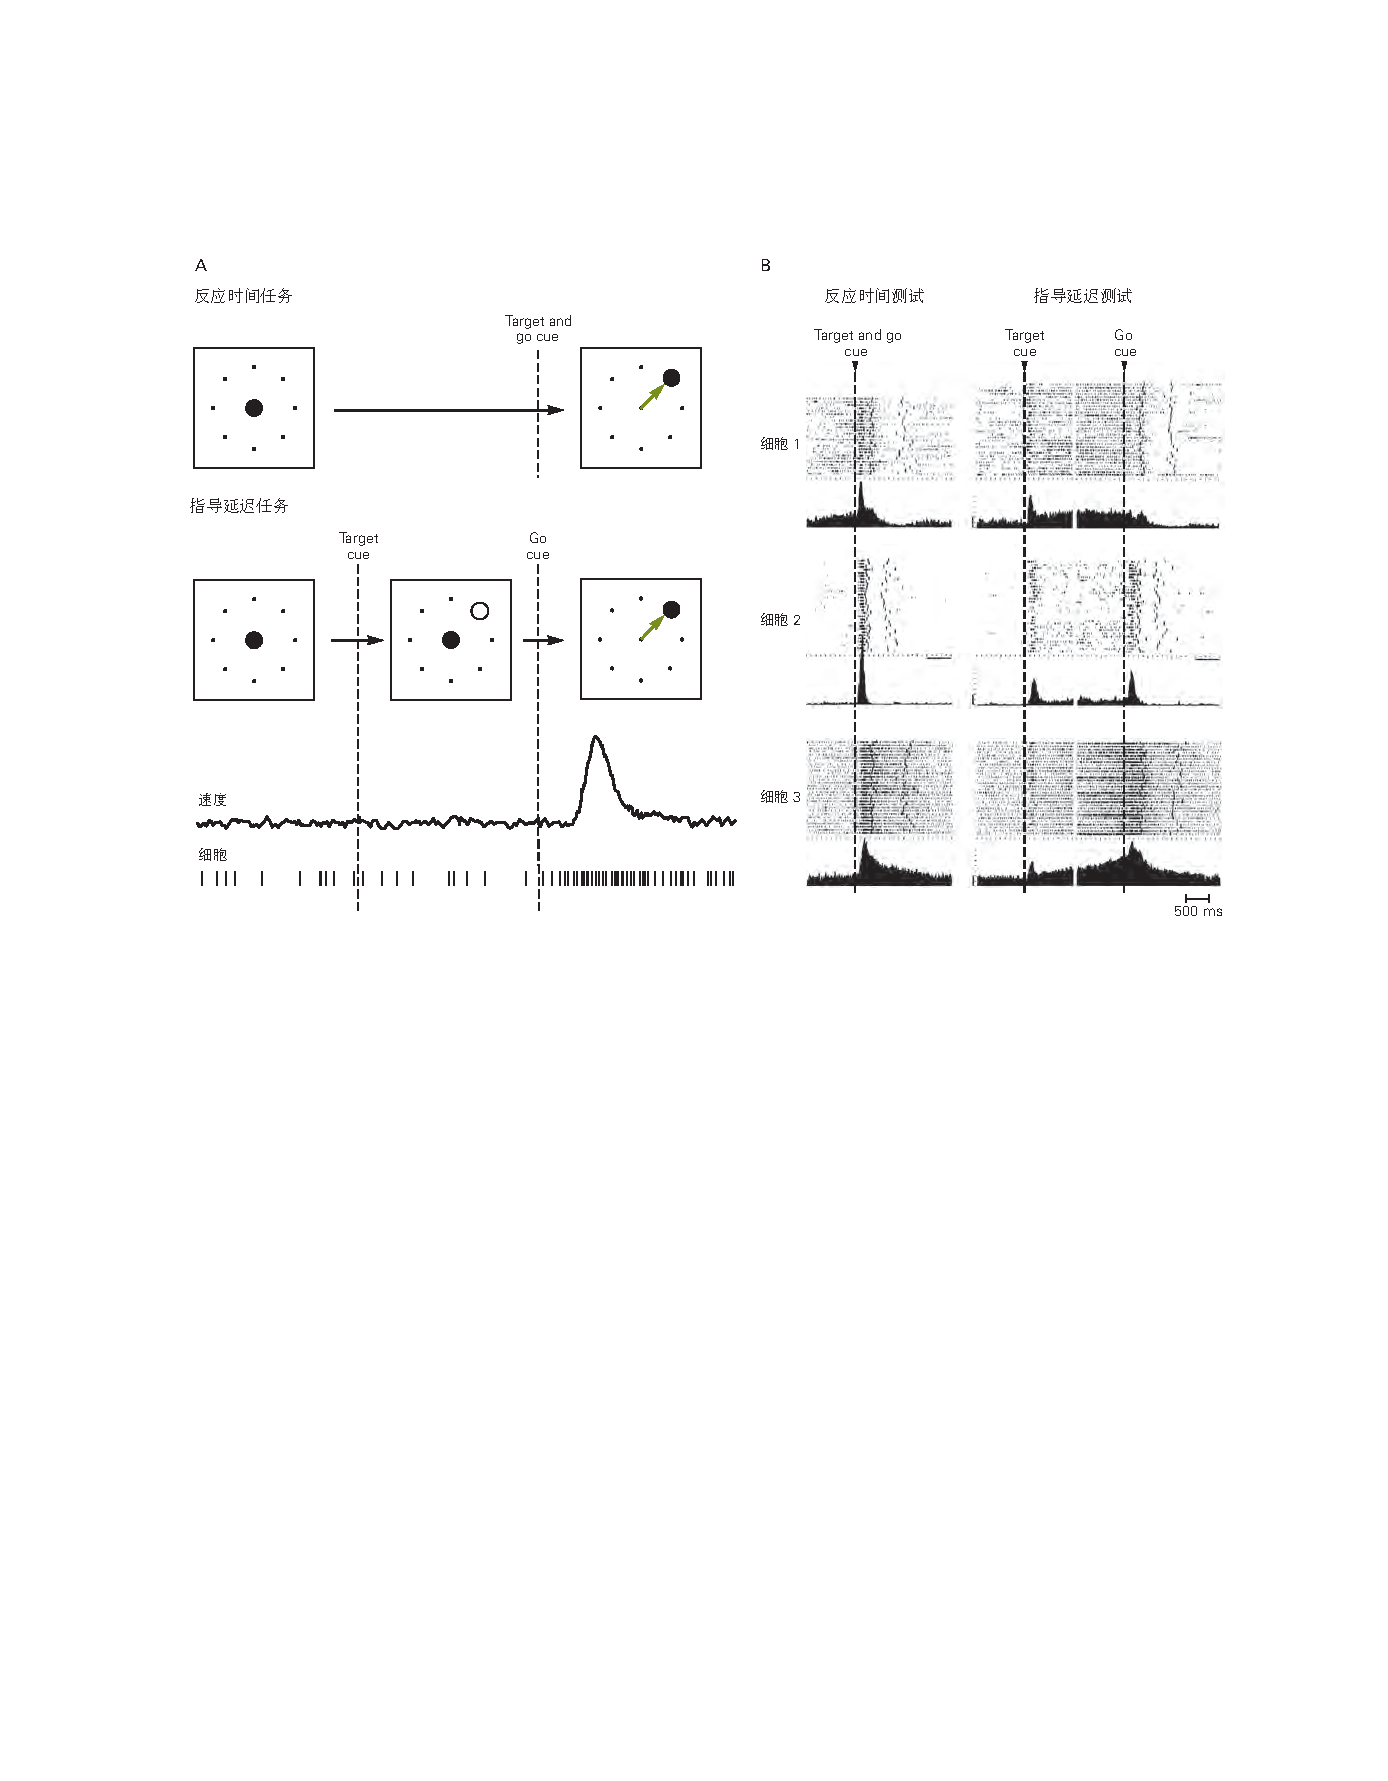
\includegraphics[width=1.0\linewidth]{chap34/fig_34_4}
	\caption*{与运动规划和运动执行相关的神经过程可以及时分离。 (经许可转载自 Crammond 和 Kalaska 2000。)
	A. 在反应时间任务中,感官提示指示受试者移动到哪里(目标提示)和何时移动(去提示)。 计划和启动运动执行所需的所有神经操作都在提示出现和运动开始之间的短暂时间内执行。 在指示性延迟任务中,初始提示告诉受试者移动到哪里,然后才给出开始提示。 第一个提示提供的知识允许主体计划即将到来的动作。 在第一个提示之后但在第二个提示之前发生的任何活动变化都被认为是计划阶段的神经相关因素。
	B. 运动计划和执行在给定皮层区域的单个神经元或神经群水平上并未完全分离。 光栅图和累积直方图显示三个前运动皮层神经元在反应时间试验和指示延迟试验期间对每个细胞首选方向运动的反应。 在栅格图中,每一行代表单个试验中的活动。 每个光栅行中的细抽动表示动作电位,两个较粗的抽动表示运动的开始和结束。 在反应时间试验中,猴子在目标出现之前不知道向哪个方向移动。 相比之下,在指示延迟试验中,初始提示会在第二个信号出现之前通知猴子目标所在的位置,以启动运动。 在延迟期间,许多运动前细胞的活动显示出定向调整的变化,表明即将发生的延迟运动的方向。 单元格 1 中的活动似乎与任务的计划阶段密切相关,因为在指示延迟任务中,在发出信号后没有执行相关的活动。 其他两个单元格显示与计划和执行相关的不同程度的活动。}
\end{figure}


\section{顶叶皮层提供有关世界和身体的信息,用于状态估计以计划和执行电机动作}
感官信息对于选择适当和有效的行动至关重要。 在从杯子喝水之前,大脑会使用视觉输入来识别哪个物体是杯子,它相对于身体的位置,以及它的物理特性,如大小、形状和手柄方向。 此外,有关手臂和手的当前姿势和运动的信息是通过将来自肢体的本体感受信号与运动命令的效应副本相结合来提供的(第 30 章)。 最后,皮肤信号在与物体进行手动交互时至关重要,例如抓住和举起杯子。

几行证据表明顶叶皮层是运动动作感觉处理中的关键大脑区域。 顶叶,尤其是 PE、PEip 和 MIP,从 S-I 接收关于身体姿势和运动的强烈躯体感觉输入。 IPS 沿线和 IPS 内的几个顶叶区域是背侧视觉通路的主要组成部分,它处理有关物体的视觉空间信息,这些物体在伸手、抓住和操纵它们时引导手臂和手的运动。 顶叶也与中央前皮质运动区相互连接,为中央前皮质提供运动感觉引导信号,并从相同的中央前区接收运动命令的输出副本。 最后,患有后顶叶皮层病变的人类受试者通常在使用感觉信息指导运动动作时表现出特定的障碍(方框 34-1)。


\subsection{顶叶皮层将感觉信息与运动动作联系起来}
我们将周围的空间体验为一个单一的统一环境,在这个环境中,物体相对于彼此和我们自己都有特定的位置。 经典神经学认为,顶叶通过整合来自不同感觉方式的输入,构建了一个统一的多模态神经表征世界。 这张单一的空间地图被认为提供了空间感知和运动的感官引导所需的所有信息,因此由控制身体不同部位(如眼睛、手臂和身体)的不同运动电路共享。 手。

然而,认为顶叶皮层包含单一地形组织空间表征的想法是不正确的。 相反,后顶叶皮层包含几个不同的功能区域,它们并行工作并接收与不同效应器(例如眼睛、手臂和手)的运动引导相关的感觉和运动输入的不同组合。 这些区域的神经元通常是多模式的,具有视觉和躯体感觉感受野,并且在特定效应器运动之前和运动期间优先放电。 每个功能区域都连接到参与控制相同效应器的额叶运动区域。 最后,每个区域都不是按照熟悉的周围空间的忠实点对点表示的拓扑结构组织的,而是包含具有不同感觉输入的神经元的复杂混合物,这些神经元可能有助于引导运动动作所需的多感觉整合 环境。



\subsection{身体位置和运动在后顶叶皮层的几个区域表示}
S-I 和相邻的上顶叶皮层区域 PE、MIP 和 PEip 是关于身体部位的位置和运动的本体感受和触觉感觉信息的主要来源。 S-I 区域 1 和 2 中的神经元通常对来自对侧身体有限部分的触觉输入或一个或几个相邻关节在特定方向上的运动做出反应。

相反,许多 PE 和 MIP 神经元在多个关节的被动和主动运动期间放电。 一些细胞也会在多个身体部位的联合运动中做出反应,包括双臂的双边运动。 许多 PE 和 MIP 神经元也有较大的触觉感受野,其反应受肢体运动或姿势期间的情境调节。 例如,具有覆盖手的整个无毛(手掌)表面的触觉感受野的神经元可能仅在手靠近身体时才对与物体的物理接触做出反应,而不是当它用手臂完全接触物体时 扩展。

这些发现表明,虽然区域 1 和区域 2 神经元对特定身体部位的位置和运动进行编码,但上顶叶神经元整合了有关各个关节位置以及肢体节段相对于身体的位置的信息。 这种集成创建了一个神经“身体图式”,它提供了关于手臂相对于身体的位置以及不同的手臂部分如何相对于彼此定位和移动的信息。 这种身体模式对于选择如何实现行为目标和持续控制运动至关重要。

例如,有效伸手的关键要求是了解手臂在伸手之前和期间的位置。 在 Brodmann 区 2 和邻近的上顶叶小叶(区域 5 或 PE)有实验性损伤的猴子在没有视觉的情况下,在本体感受和触觉引导下,无法触及和操纵物体。 具有类似病变的人类患者表现出相同的缺陷,没有空间忽视,这是下顶叶更多横向病变的常见结果。


\subsection{空间目标在后顶叶皮层的几个区域都有体现}
IPS 内的功能区域与空间信息的处理密切相关,尤其是与行动相关的视觉信息。 这些区域中的每一个都有独特的方式来表示相对于身体的物体和空间目标,并有助于控制身体不同部位的运动动作。 例如,外侧顶内区域 (LIP) 中的许多神经元接收来自纹状体皮质区域的视觉输入。 它们的感受野固定在视网膜坐标中,并在猴子改变注视方向时转移到新的空间位置。 当动物注意到感受野内的刺激时,即使不看它,神经反应也常常会增加,并且它们通常会在针对它们感受野中的视觉刺激的眼跳之前放电(图 34-5A;参见第 1 章) 35).

几个顶叶区域优先参与手臂和手部运动的控制。 例如,上顶叶皮层的最内侧区域 V6A 和 PEc 区域接收来自纹状体外视觉区域 V2 和 V3 的输入。 许多 V6A 和 PEc 神经元在视网膜坐标中具有视觉感受野,但它们的活动也经常受到注视方向、当前手臂姿势和伸手动作方向的调节。

IPS 底部的腹侧顶内区 (VIP) 接收来自背侧视觉流的两个组成部分的输入,即内侧颞叶皮层和内侧颞上皮层,它们参与光流和视觉运动的分析。 许多 VIP 神经元对视觉刺激和体感刺激做出反应,其感受野位于面部或头部,在某些情况下,还位于手臂或躯干上。 神经活动处于以头部为中心的坐标中,因为即使眼睛移动以注视不同的空间位置,体感和视觉信息仍保持在记录中(图 34-5B)。 一些 VIP 神经元对沿同一方向移动的视觉和触觉刺激都有反应,而其他神经元则被向其触觉感受野移动的视觉刺激强烈激活,但前提是运动路径最终会与触觉感受野相交。 这些神经元可以让猴子将物体在他们直接的周围空间中的位置和运动与他们身体的不同部位联系起来。

与到达相关的顶叶皮层的另一个区域是顶叶到达区域 (PRR)。 PRR 可能对应于内侧顶内皮层 (MIP) 和相邻的上顶叶皮层和下顶叶皮层的臂控制部分。 许多 PRR 神经元的活动随着到达目标相对于手的位置而变化。 然而,此信号并未固定在手或目标的当前位置,而是固定在当前注视方向(图 34-5C)。 每次猴子朝不同的方向看时,PRR 神经元的触及相关活动都会发生变化,即使目标和手的位置以及所需的触及轨迹没有改变。 相比之下,PE 和 PEip 区域中许多神经元的触及相关活动与注视的相关性较低,而与当前手部位置和手臂姿势的相关性更强。 与 PRR 相比,PE 和 PEip 神经元因此提供了关于相对于手的当前位置的到达目标位置的更稳定的信号。

最后,前顶内区 (AIP) 中的神经元主要涉及通过手的运动来抓取和操纵物体。 许多 AIP 神经元在伸手去拿和抓住特定形状、大小和空间方向的物体时优先活跃,甚至经常在抓住它们之前查看这些物体时(图 34-5D)。 神经反应特性范围很广,从几乎只对物体的视觉输入做出反应但对抓取动作没有反应的神经元,到即使在黑暗中也只在手部运动时放电的神经元。 这表明 AIP 包含神经回路,这些神经回路开始将有关物体物理特性的视觉信息(与处理方式相关)——詹姆斯·吉布森 (James Gibson) 称之为物体的可供性——转化为适当的手部动作(第 56 章)。

关于顶叶皮层的一个有趣发现是,神经元的感受野可以通过个人经历(例如工具使用)而改变。 训练猴子使用耙形工具取回手臂和手正常够不到的食物颗粒。 许多 VIP 神经元通常会对位于手的当前位置附近或手臂可触及的任何地方的视觉对象做出反应。 训练后,当猴子抓住工具时,它们的视觉感受野会瞬时扩大以吸收工具,就好像工具的远端已经成为猴子自己手和手臂的功能延伸(图 34-6)。


\subsection{内部产生的反馈可能影响顶叶皮层活动}
将手臂运动的视觉和躯体反馈从外周传递到皮层回路的延迟会导致实时感觉运动控制的振荡甚至不稳定。 这个问题的一个理论解决方案是使用前向内部模型,根据传出运动命令的内部效应副本以及较慢的外围反馈信号(第 30 章)对身体运动进行预测估计。

几行证据表明,顶叶皮层回路和小脑(第 37 章)可能实现类似的解决方案。 PE、MIP 和 PRR 中的许多与到达相关的神经元不仅在响应被动感觉输入时活跃,而且在运动开始之前和延迟到达任务的指示延迟期间也是活跃的。 这些反应表明这些神经元在运动开始之前处理集中生成的关于运动意图的信号。 这种运动前活动通常被解释为顶叶皮层产生有助于早期运动规划的前馈信号的证据。 然而,另一种解释是运动前活动是由预期运动的运动命令的输出副本驱动的,该运动命令通过与中央前运动区域的相互连接传输到顶叶皮层。 这种外周感觉输入和中央效应副本的组合可以允许一些与顶叶触及相关的电路计算对手臂当前状态及其相对于行为目标的位置的持续更新估计。 该估计可用于快速纠正正在进行的手臂运动中的错误。

顶叶回路是主要参与受试者运动意图的形成还是状态估计将取决于其运动前活动的起源。 如果它主要在顶叶皮层本身内产生,这将强烈暗示顶叶皮层参与了预期运动的规划。 相比之下,如果它主要由从中央前运动区域中继的输出副本驱动,这将强烈暗示顶叶回路参与状态估计,包括预测手臂应如何响应运动命令而移动。



\section{前运动皮层支持运动选择和规划}
正如本章开头所概述的,在给定情况下以特定方式采取行动的决定取决于许多因素,包括关于物体、事件的感官信息,以及来自环境的行动机会、身体姿势和运动、内部动机 状态、先前的经验、奖励偏好以及将感官输入与运动动作联系起来的任意规则和策略。 您想喝咖啡的原因可能有很多,而这种愿望可以通过各种行动来满足,从简单地伸手拿满满的咖啡杯到在家煮咖啡或去咖啡馆。

位于 M1 喙侧的额叶前运动皮层区域在早期运动规划或任务选择过程中起着重要作用。 这些区域中的许多神经元,例如图 34-4 中所示的 PMd 神经元,在指令延迟任务期间产生活动,这些任务反映了猴子的运动意图,甚至是影响这些动作选择的因素。 不同的运动前皮层区域被认为对运动选择和规划做出不同但重叠的贡献。 例如,包括 PMd 和 PMv 在内的外侧前运动皮层传统上与外部感觉输入启动和引导的动作有关。 相比之下,内侧运动前区,包括 SMA、前 SMA 和 CMA,与自发运动的控制以及动作的抑制有关。 然而,他们各自贡献的区分并不是绝对的。


\subsection{内侧前运动皮层参与自主行为的情境控制}

克林顿·伍尔西 (Clinton Woolsey) 开创性的电刺激研究表明,除了 M1 中的运动图之外,额叶皮层的内侧壁还包含一系列神经元,这些神经元也可以调节身体运动。 这个内侧运动图,现在称为辅助运动区 (SMA),包括整个对侧身体,但比 M1 中的详细图更粗糙,如后所述。 需要强大的刺激电流来唤起运动,这些运动通常是复杂的动作,例如姿势调整或踏步和攀爬,并且可能涉及身体的两侧。 今天,人们一致认为该区域包含两个具有不同细胞构造特征、轴突连接和功能特性的区域:更尾端的 SMA 本身和更延髓的前辅助运动区 (pre-SMA),我们统称为辅助运动区 皮层(SMC)。

SMC 涉及自愿行为的许多方面,尽管它的贡献仍然存在争议。 几行证据支持自发行为中的作用。 在人类中,低于运动启动阈值的 SMC 电刺激可以唤起内省的运动冲动感,这种感觉在 M1 刺激期间不会出现。 SMC 的损伤会产生启动所需运动或抑制不需要的运动的问题(方框 34-2)。 此外,在执行自定进度运动期间颅骨表面的慢皮层电位记录表明,初始电位在运动开始前 0.8 到 1.0 秒出现在额叶皮层中。 该信号称为准备电位,在以 SMC 为中心的皮层中达到峰值。 因为它发生在运动之前,所以准备潜能被广泛解释为该区域的神经活动参与形成运动意图的证据,而不仅仅是执行运动。

SMA 和前 SMA 中的神经元在自主运动之前和期间放电。 与 M1 神经元不同,大多数 SMA 神经元的活动与身体部位的特定动作没有那么紧密地耦合,而是似乎与手、手臂、头部或躯干的更复杂、协调的运动动作相关联。 与 SMA 神经元相比,前 SMA 神经元通常在运动开始之前更早开始放电,并且与运动执行的耦合度较低。

SMC 与所谓的行为执行控制有关,例如在不同的行动、计划和策略之间切换所需的操作。 例如,在猴子中,当受试者收到指示其改变运动目标或抑制先前计划的运动的提示时,一些 SMC 神经元会强烈放电。 因此,SMC 可能包含一个系统,可以在它们不再适用时覆盖电机计划。

SMC 还涉及运动序列的组织和执行。 一些 SMC 神经元在特定的三个动作序列开始之前放电,但在相同的三个动作的不同序列之前不放电(图 34-7)。 其他神经元仅当特定运动发生在序列中的特定位置时或当发生特定的连续运动对而不管它们在序列中的位置如何时才会放电。 相比之下,一些其他的 SMC 神经元仅在猴子进行序列的特定顺序位置(例如,仅第三个)发生的运动时放电,而不管其性质或序列中仍有多少运动要执行。

这些看似不同的功能可能反映了 SMC 在自愿行为的情境控制中更普遍的作用。 情境控制涉及根据内部和外部线索的不同组合选择和执行那些被认为适当的行动,以及在特定环境或社会背景下阻止不适当的行动。 它还可能涉及组织实现特定目标所需的行动顺序。 上下文控制可能还涉及其他神经回路的贡献,例如前额叶皮层和基底神经节区域。

扣带回运动区 (CMA) 也可能有助于行为的情境控制。 CMA 似乎参与了在运动错误后选择替代行动或响应不断变化的奖励意外事件。 例如,猴子被训练去推动或转动手柄以响应非指导性的触发信号。 最初,如果猴子在连续试验中做出相同的动作(推动或转动手柄),它们将获得大量奖励。 经过几次试验,奖励的大小开始减少。 如果猴子随后切换到另一个动作,则在多次试验重复该动作后,奖励大小会恢复到最大值。 因此,对猴子来说,最好的策略是,一旦它们检测到奖励量减少,就在重复推动或转动手柄之间切换。

在这项任务中,在接受奖励和开始下一次试验之间的间隔期间,头端 CMA 中的一些神经元会做出反应。 在奖励减少的试验中,当猴子在下一次试验中做出相同的动作时,这些神经元中与任务相关的活动没有改变; 只有当猴子在下一次试验中切换到另一种运动时,它们的活动才会发生变化。 重要的是,当视觉提示指示猴子在下一次试验中改变动作时,这些相同的神经元并没有表现出相同的反应变化。 这表明这些延髓 CMA 神经元优先参与基于行动结果(奖励大小)切换和移动到替代目标的自愿决定,而不是通过视觉指令进行切换。


\subsection{背侧前运动皮层参与规划手臂的感觉引导运动}
Ed Evarts、Steven Wise 及其同事在 1980 年代进行的记录研究表明,外侧前运动皮层(包括 PMd 和 PMv)在感觉引导运动的选择和规划中起着至关重要的作用。 这些研究表明,许多前运动神经元会发出短暂的短潜伏期放电爆发,以响应发出特定动作信号的指令提示,或在指令提示出现和允许指令动作的第二个提示之间的指示延迟期间持续活动( 图 34-4)。

该活动反映了有关预期行为的信息,包括目标的空间位置、手臂运动的方向和其他运动属性。 重要的是,PMd 延迟期活动可以反映用对侧或同侧手臂到达特定位置的意图,即使两个手臂运动的生物力学细节非常不同。 这表明在与运动规划的感觉运动坐标转换模型的预测一致的外部空间坐标框架中,PMd 活动可以发出独立于用于产生动作的效应器产生运动动作的意图。 成像研究同样发现了在人类前运动皮层中用任何一只手制作的手指敲击序列的外部空间表征的证据。

从多种备选方案中选择适当的行动是自愿控制的一个关键方面。 PMd 中的延迟期活动可以反映该过程。 例如,在一项实验中,在一项任务中,猴子的 PMd 神经元进行了记录,在该任务中,动物首先收到两种颜色的空间线索,这些线索确定了两个可能到达相反方向的目标。 经过一段记忆延迟期后,位于中央的新颜色提示会告知猴子哪些空间提示是正确的目标。 在第一个指令之后,PMd 中的神经活动发出两种潜在触及动作的信号,但在第二次指令之后,PMd 中的神经活动立即只发出猴子触及选择的信号(图 34-8A)。 这表明 PMd 可以在最终决定采取哪个动作之前准备多个潜在的运动动作。 随后的研究表明,这可能仅限于不超过三到四个同时发生的潜在行动。 顶叶区域 PRR 中的伸展相关神经元也有助于在做出最终动作决定之前准备两个潜在的运动动作(图 34-8B),揭示该过程如何分布在多个与手臂运动相关的皮层神经群中。

PMd 神经元也可以发出故意决定不移动的信号。 当目标位置的彩色视觉提示指示猴子到达目标时,许多 PMd 神经元在指示延迟期间产生定向调谐活动,但当同一位置的不同颜色提示指示猴子不要到达目标时,它们的活动会减少 到达它。 这种不同的活动是一个明确的信号,在动作执行前几秒,关于猴子打算朝特定方向到达还是不移动以响应指令提示(图 34-9)。 有趣的是,在同一任务中研究的顶叶区域 PE/MIP 中的许多神经元在延迟期间继续产生定向调谐活动,即使在指令提示停止到达之后,这表明顶叶皮层保留了潜在动作的表征,而这些动作最终不会 执行。

前运动皮层中的许多神经元也在运动执行过程中放电。 鉴于与计划和执行相关的活动如此接近,即使在单个神经元的水平上,一个主要问题是为什么与计划相关的神经活动不会立即启动运动。 是什么阻止运动过早执行? 似乎与计划相关的活动并没有简单地超过启动运动所需的最低阈值,也没有出现必须释放以允许运动开始的单独的明显制动机制。

一种不同的解释在规划和执行到达过程中的神经处理的方法可能会从动力系统的角度为这些问题提供答案。 这个想法是,皮层运动回路形成了一个动态系统,其分布式活动模式随时间演变为初始状态、输入信号和随机神经反应可变性(“噪声”)的函数。 因此,计划和执行的不同阶段的活动模式反映了网络的不同状态,包括延迟期间可以准备运动但不激活肌肉的特定状态(图 34-10)。 在同一运动的重复过程中,群体水平活动模式的总体相似性表明,在运动的计划和执行过程中,整个群体经历了一种协调的活动共同调节模式,由神经回路内的突触连接决定。


\subsection{背侧前运动皮层参与应用管理行为的规则(关联)}
行为通常受任意规则的指导,这些规则将特定的符号提示与特定的动作联系起来。 开车时,您必须根据交通灯是绿色、黄色还是红色执行不同的操作。 在已经学会将任意提示与特定动作联系起来的猴子中,运动前区的许多细胞有选择地对特定提示做出反应。 例如,为了在图 34-8 中的双目标研究中选择正确的目标,猴子必须应用一个规则,将颜色映射到由两个连续的指令提示提供的目标位置。

PMd 涉及新的运动相关关联或规则的获取。 在一项实验中,当猴子学习四种不熟悉的视觉线索和四种不同的运动方向之间的关联时,PMd 神经元会进行记录。 虽然猴子的选择最初是随机的,但他们在几十次试验中学会了规则。 猴子响应每个提示做出手臂运动; 在学习的早期“猜测”阶段,许多 PMd 神经元的活动较弱,但随着猴子学习哪个提示表示哪个动作,强度和定向调节逐渐增加。 随着规则的获得,其他神经元的活动也相应下降。 学习过程中活动的这些变化既反映了动作选择,也反映了对将提示与动作联系起来的规则的知识水平不断提高。

规则的性质也会对神经反应产生强烈影响。 在经过训练的猴子中,它们可以根据空间规则(视觉提示的位置)或语义规则(提示的任意指定含义与其位置无关)在几种可能的运动之间进行选择,许多前额叶和 PMd 神经元在动物时优先活跃 选择使用一个规则而不是另一个规则的运动。 这表明神经活动不仅与特定提示或动作有关,还与它们之间的关联有关。

运动前区甚至参与抽象规则的实施。 例如,猴子接受了一项任务的训练,该任务需要两个决策,一个是感知决策,另一个是行为决策,而这两个决策之前没有关联。 在每次试验中,猴子首先必须决定两个顺序呈现的视觉图像是相同还是不同(匹配/不匹配的感知决定)。 在一些试验中,与样本视觉图像同时出现的规则提示指示猴子在两个图像相同时移动它们的手,并且在它们不同时避免移动(走/不走运动决定); 在其他试验中,规则是相反的——如果图像不同就移动,如果图像匹配就不要移动。 在呈现测试视觉图像后,PMd 中的神经活动与运动决策的相关性比每次试验中的感知决策更强,但两种决策均以 PMd 表示。 更引人注目的是,在测试图像出现后引导运动决策的两个视觉图像之间的延迟期间,PMd 活动还与匹配/不匹配行为规则相关(图 34-11)。 这些结果表明,PMd 在应用管理行为适当性的规则以及根据现行规则做出行为决策方面发挥着重要作用。 在同一任务(未显示)中,前额叶皮层的神经记录发现视觉图像的物理身份有很强的表现,但与 PMd 相比,行为规则和运动决策的相关性较弱且较晚。



\subsection{腹侧前运动皮层参与规划手的运动动作}
前运动皮层的最外侧部分,区域 PMv,与顶叶皮层区域 AIP、PF 和 PFG 以及次级体感区域相互连接。 电刺激显示 PMv 包含广泛重叠的电路,可控制手和嘴的运动。

与 AIP 神经元一样,许多 PMv 神经元似乎有助于根据目标对象提供的物理功能来控制手部动作。 这些神经元倾向于在某些刻板的手部动作(例如抓握、握住、撕裂或操纵物体)期间优先放电。 许多神经元只有在猴子使用特定类型的抓握时才会放电,例如精确抓握、全手抓握或手指抓握(图 34-12)。 精确抓握是最常出现的类型。 一些 PMv 神经元在整个动作过程中放电,而其他神经元在一种抓握的特定阶段选择性放电,例如在手指张开或闭合期间。

PMv 神经元的另一个显着特性是它们的放电通常与运动行为的目标相关,而不是与形成它的个体运动相关。 因此,当用右手、左手甚至嘴巴等不同的效应器执行抓取物体时,许多 PMv 神经元会放电。 相反,当食指弯曲以抓住物体时,PMv 神经元可能活跃,但当动物弯曲同一根手指抓挠自己时,PMv 神经元可能不活跃。


\subsection{前运动皮层可能有助于指导运动行为的知觉决策}
一系列研究提供的证据表明,皮层运动区不仅代表指导随意运动的感觉信息,而且还表达做出和执行知觉决定所必需的神经操作。 猴子被训练来区分施加在一根手指上并在时间上相隔几秒钟的两次短暂振动刺激之间的频率差异。 动物必须决定第二个刺激的频率是高于还是低于第一个,并通过伸出手用另一只手按下两个按钮中的一个来报告它们的感知决定。

该任务中的决策过程可以被认为是一系列神经操作:(1)在第一个刺激频率(f1)出现时对其进行编码; (2) 在两次刺激之间的间隔期间,在工作记忆中保持 f1 的表征; (3) 在出现时对第二个刺激频率 (f2) 进行编码; (4) 将f2与f1的内存轨迹进行比较; (5)判断f2的频率是高于还是低于f1; 最后,(6) 使用该决定来选择另一只手的适当动作。 最后一步之前的一切似乎都完全属于感官辨别处理的范围。

当猴子执行任务时,初级 (S-I) 和次级 (S-II) 体感皮层中的神经元会在刺激出现时编码它们的频率。 在 f1 和 f2 之间的间隔期间,表示记忆的 f1 的 S-I 中没有持续的活动,只有 S-II 中的短暂表示,它在 f2 出现之前消失了。

然而,引人注目的是,前额叶皮层、SMC 和 PMv 中许多神经元的活动在传递时与 f1 和 f2 的频率成比例。 此外,一些前额叶和运动前神经元在 f1 和 f2 之间的延迟期间表现出与 f1 频率成正比的持续活动。 最值得注意的是,这些区域中的许多神经元,尤其是 PMv 中的神经元,在传递 f2 时独立于它们的实际频率对 f2 和 f1 之间的频率差异进行编码(图 34-13)。 这个集中生成的信号适合调解决定按下哪个按钮的知觉辨别力。 编码 f2-f1 差异的神经元在 S-I 中不存在,并且在 SMC 和 PMv 中比在 S-II 中更常见。


\subsection{当观察到其他人的运动动作时,几个皮层运动区会活跃}
一些运动前区和顶叶区可以在没有明显的动作意图时被激活,例如当一个人被要求想象执行某种运动动作时。 这种现象被称为运动想象,已经在使用功能性脑成像的人类中得到证实。 运动想象诱发的神经活动可能反映了与运动计划和准备相关的大脑机制,这些机制与其公开执行无关。

皮层运动回路在没有明显行动的情况下被激活的第二种情况是,当一个人观察到另一个人执行作为她自己的运动曲目一部分的运动行为时。 对行为和社交互动的控制在很大程度上取决于识别和理解他人正在做什么以及他们为什么这样做的能力。 这种理解可能来自对观察到的行为的性质进行高阶视觉感知分析,并根据自己的经验推断出行为的动机和目的。 另一种解释是直接匹配假设,即观察他人的行为会激活观察者体内控制类似运动行为的运动回路。 根据这一假设,运动回路的同理心激活可以在观察到的行为与观察者存储的关于他们过去执行的类似行为的性质、动机和后果的知识之间建立联系。

支持直接匹配假说的显着证据是通过发现称为镜像神经元的大量神经元提供的,首先是在 PMv 中,后来是在猴子的顶叶 AIP 中。 当猴子主动抓取和操纵物体时,以及当它观察到另一只猴子或实验者执行的类似动作时,镜像神经元都会放电(图 34-14)。 当猴子简单地观察潜在的目标物体或在没有目标物体的情况下观察模仿的手臂和手部动作时,镜像神经元通常不会做出反应。 一些顶叶镜像神经元甚至可以区分观察到的类似动作的最终目标,例如抓取和捡起食物来吃还是把它放进杯子里。

神经记录和大脑成像研究表明,人类也被赋予了一种类似镜子的机制,可以将观察到的动作与编码在他们的运动系统中的动作相匹配。 这种活动出现在皮层的各个区域,包括头侧顶下小叶、IPS、PMv 和额下回后部。

皮质运动回路似乎参与理解和预测观察到的事件的结果。 在一项实验中,当猴子只是在监视器上观看相同的提示和光标运动而看不见的一方执行任务时,参与使用视觉提示选择到达目标的 PMd 神经元(图 34-8)也会放电。 当光标移动到正确的目标时,猴子会获得免费的果汁奖励,但如果移动到错误的目标,则不会。 在果汁实际输送之前光标开始移动到正确的目标后不久,猴子开始舔果汁管,但当光标移向错误的目标时,猴子很快将嘴从管子上移开。 这种行为表明猴子正确地解释了他们所看到的并准确地预测了其后果。

值得注意的是,无论猴子是使用视觉线索来计划和进行手臂运动,还是只是观察视觉事件并预测其结果,大多数与任务相关的 PMd 神经元的活动都惊人地相似。 如果在正确的试验后没有提供奖励,或者如果动物吃饱了并且对喝果汁不感兴趣,那么这些神经元会在观察期间停止响应。 这表明神经元不仅仅是对感官输入做出反应,而是在处理观察到的感官事件以预测它们对猴子的最终结果,即免费果汁奖励的可能性。

这种与被动观察相关的激活支持这样一种观点,即在非运动环境中激活前运动电路可能有助于理解环境中观察到的事件的性质和后果。 它也与人类受试者仅通过观察熟练的人执行相同的动作来学习新的运动技能的能力有关。 此外,幼儿镜像神经元系统的功能障碍可能会导致自闭症的某些症状。

\subsection{自主控制的许多方面分布在顶叶和前运动皮层}
虽然我们已经分别描述了顶叶和中央前皮层运动前区的作用,但必须强调的是,主要的感觉运动控制过程通过相互联系在多个皮层区域共享。

例如,将目标对象的物理可供性与适当的手部动作联系起来的神经过程分布在顶叶区 AIP、运动前区 PMv 和 M1 中,该过程的视觉空间方面在 AIP 中更为突出,而运动成分在中央前皮层中更为普遍 (图 34-15)。 同样,如前所述,PRR 中到达目标选择的神经相关性(图 34-8B)与 PMd 中报告的那些(图 34-8A)惊人地相似。



\section{初级运动皮层在运动执行中起着重要作用}
一旦一个人决定了行为目标,就必须将运动命令传达给肌肉以移动身体。 不能低估这个问题的复杂性,因为它需要精确控制作用于许多关节的大量肌肉活动的时空模式以实现行为目标,同时还要考虑肌肉骨骼系统和力的复杂非线性机械特性 和环境施加的负载。 这些肌肉活动的详细模式由脊髓运动神经元和神经元间回路协调(第 32 章)。 然而,初级运动皮层 (M1) 在生成控制脊柱活动的运动命令方面起着重要作用,包括选择和控制肌肉活动的时间和幅度所需的基本信息。


\subsection{初级运动皮层包括运动外围的详细地图}
大脑皮层的局部区域包含专门用于自愿运动控制的身体运动图的想法可以追溯到 19 世纪中叶英国神经学家约翰休林斯杰克逊的工作。 他在治疗癫痫发作患者时得出了这个结论,这些患者的特征是反复出现痉挛性不自主运动,有时类似于有目的的随意动作的片段,并且在每次发作期间系统地发展到包括身体的不同部位(第 58 章)。 在 19 世纪后期,改进的麻醉和无菌手术技术允许对实验动物的大脑皮层进行直接实验研究。 使用这些新方法,柏林的 Gustav Fritsch 和 Eduard Hitzig 以及英国的 David Ferrier 表明,对不同麻醉哺乳动物物种的有限区域皮质表面进行电刺激会引起对侧身体部分的运动。 在猴子身上,引起运动所需的电流在沿着中央沟头侧岸的一条窄带中最低,该区域现在被称为初级运动皮层。

他们的实验表明,在这条组织带内,对相邻部位的刺激会引起相邻身体部位的运动,从内侧的脚、腿和尾巴开始,然后向外侧延伸到躯干、手臂、手、脸、嘴和舌头。 当他们损伤皮层部位时,刺激会引起身体一部分的运动,在动物从手术中恢复后,该身体部位的运动会受到干扰或消失。 这些早期实验表明,运动皮层包含对侧身体主要部分的有序运动图,并且运动图的完整性对于相应身体部位的自主控制是必要的。 20 世纪上半叶,克林顿·伍尔西 (Clinton Woolsey) 对许多物种的研究以及怀尔德·彭菲尔德 (Wilder Penfield) 对接受手术的人类的研究表明,中央沟的头侧岸的一般地形组织在许多物种中都是保守的(图 34-16)。 一个重要的观察结果是,运动图并不是身体解剖形态的精确点对点再现。 相反,最精细控制的身体部位,如手指、面部和嘴巴,由不成比例的大区域表示,反映出精细运动控制所需的大量神经元。

如今,地图上研究得最好的区域是那些控制手臂和手的部分,它们揭示的复杂性远远超过图 34-16A、B 中显示的经典图表中传达的复杂性。 首先,控制手指、手和远端手臂肌肉的神经元往往集中在中央区域,而控制更近端手臂肌肉的神经元则位于中央核心周围的马蹄形环中(图 34-16C)。 其次,刺激部位广泛重叠,可以控制作用于不同关节的肌肉; 相反,每块肌肉都可以通过刺激分散在手臂/手部运动图上的许多部位来激活。 最后,局部水平轴突连接连接运动图上的不同位点,可能允许在运动指令形成期间协调整个图上的活动。


\subsection{初级运动皮层中的一些神经元直接投射到脊髓运动神经元}
如前所述,虽然灵长类动物中的许多皮质脊髓轴突仅终止于脊髓中间神经元,但其他人也直接与脊髓运动神经元形成突触。 这些皮质运动神经元 (CM) 细胞仅存在于 M1 的最尾部,位于中央沟的前岸。 投射到支配不同肌肉的脊髓运动神经元池的 CM 细胞分布存在广泛重叠(图 34-17A)。

CM 细胞在非灵长类物种中非常罕见或不存在,并且在从原猿类动物到猴子、类人猿和人类的灵长类动物系统发育过程中逐渐成为皮质脊髓束的重要组成部分。 在猴子中,更多的 CM 细胞投射到手指、手和腕部肌肉的运动池,而不是投射到手臂更近端部位的肌肉。 CM 细胞轴突的末端通常在几种不同的主动肌的脊髓运动神经元上分支和终止,并且还可以通过脊髓中间神经元上的突触影响更多肌肉的收缩活动(图 34–17B、C)。 这种终止模式被组织起来以在主动肌和拮抗肌的肌肉场中产生协调的活动模式。 最常见的是,CM 细胞轴突直接激发几个主动肌的脊髓运动神经元,并通过脊髓抑制性中间神经元间接抑制一些拮抗肌的活动(图 34-17C)。 事实上,CM 细胞在人类中比在其他物种中更为突出,这可能是与其他哺乳动物相比,人类 M1 损伤对自主运动控制具有更深远影响的原因之一(方框 34-3)。

M1 中运动图的复杂性——如针对单个肌肉和小肌肉群的短电刺激序列以及直接和间接 M1 下行输出的解剖学和神经生理学研究所揭示的那样——显示了从 M1 到脊髓运动装置的运动命令如何能够 控制身体每个部分的运动,特别关注灵长类动物的手指、手、手臂、脸和嘴巴。

\subsection{初级运动皮层的活动反映了运动输出的许多时空特征}
如前所述,可以在多个层面上描述一个给定的动作,例如伸手去拿一个物体,从手的空间轨迹和速度到以关节为中心的因果力和肌肉活动(图 34-1A)。 代表性模型假设电机系统直接计划和控制运动的特定参数。 他们预测,不同的神经群体会在参数空间(即手或关节运动或关节肌肉扭矩)中编码预期运动,并在它们之间执行转换。 动力学模型预测,神经回路通过激活状态从当前状态到所需最终状态的变化来控制运动。 随着它们的活动随时间变化,可以在单个神经元和神经群体的活动中观察到预期运动的各种参数和特性的相关性。 然而,大多数神经元的活动反映了参数的组合,这些参数与任何特定坐标框架中的任何可识别参数都不对应。

尽管他们的假设不同,但两种观点都表明,通过研究不同神经元和不同神经结构的活动如何与不同的运动参数相关,可以推断出不同神经元和不同神经结构对运动控制的可能贡献。 自 1960 年代以来,人们对 M1 神经元的活动进行了深入研究,以试图揭示,例如,M1 是否产生有关手部运动的高级信号,或与因果力和肌肉活动更相关的较低级动力学信号。

了解 M1 产生的控制信号的性质也有助于阐明其他运动结构的作用,尤其是脊髓。 如果 M1 编码有关肌肉活动模式的特定信息,则在脊髓水平上需要较少的计算处理。 相反,如果 M1 主要编码有关预期运动的高级信息,则脊髓必须执行将此全局信号转换为肌肉活动详细模式的过程。

然而,确定 M1 如何控制运动的主要实验挑战之一是事实上所有与运动相关的参数都通过运动定律相互关联。 因此,在给定身体的初始条件(姿势、运动)的情况下,特定的肌肉力量(运动学)将引起特定的运动(运动学)。 因此,如果当一只猴子在不同方向进行伸手动作时记录神经活动,那么理论上发出空间运动方向信号的神经元也将不可避免地显示出与因果力方向的相关性。 同样,肌肉的收缩活动将与运动的空间方向系统地共同变化,即使它明显产生了因果力。 除非任务设计充分分离这些不同类别的参数,否则它将产生关于每个神经元功能作用的模糊信息。

爱德华·埃瓦茨 (Edward Evarts) 是 1960 年代第一个研究这个问题的人,他开创性地记录了猴子进行简单的手腕屈曲/伸展运动时的单神经元记录。 他使用滑轮和重物系统,向猴子的手腕施加负载,在不同的试验中将手腕拉向弯曲或伸展的方向。 这需要猴子在进行运动时改变腕部肌肉活动水平以补偿负荷。 结果,手腕运动的运动学(方向和幅度)保持不变,但动力学(力和肌肉活动)随负载而变化。

他使用微电极定位了 M1 运动图中的单个神经元,当猴子在没有外部负载的情况下进行手腕运动时,这些神经元会调节它们的活动。 在一些神经元中,它们的放电在手腕屈曲(首选运动方向)期间增加,并在伸展期间受到抑制,而其他神经元则显示相反的模式。 这种与运动相关的活动通常在主动肌活动开始前 50 到 150 毫秒开始,支持 M1 神经活动和运动之间的因果关系。 当施加负载时,许多 M1 神经元在负载抵抗其首选方向的运动时增加它们的活动,而在负载辅助运动时减少活动(图 34-18)。 神经活动的这些变化与补偿外部负荷所需的肌肉活动的变化平行。

随后的研究证实,许多 M1 神经元的活动随着肌肉力量输出的大小而系统地变化。 这在猴子对阻止运动的不可移动物体产生等距力的任务中得到了最好的体现。 许多 M1 神经元(包括 CM 细胞)的活动随单个关节(例如手腕或肘部)以及使用拇指和食指进行精确捏合时产生的静态等距输出力的方向和水平而变化(图 34) –19A). 至少在部分测试范围内,这些响应随静力水平线性变化。

大多数自然行为涉及多关节、多肌肉动作。 例如,手臂在不同方向的伸展运动需要肩部和肘部的不同模式的协调运动。 到达期间的近端肢体肌肉活动显示大致余弦活动模式,在特定运动方向上具有最大活动,其首选运动方向随着所需到达方向与肌肉首选方向之间的角度增加而逐渐减小(图 34-20A) ). 与近端手臂肌肉一样,与肩部和肘部运动相关的单个神经元在以最大活动的首选方向为中心的不同伸展方向的运动期间以连续分级的方式做出反应(图 34-20B)。 不同的神经元有不同的偏好方向,覆盖了圆圈周围的整个方向连续体,在任何给定的运动中,具有广泛偏好方向的神经元以不同的速率放电。

正如埃德·埃瓦茨 (Ed Evarts) 在单关节任务中所展示的那样,到达过程中的大部分 M1 活动都与因果动力学密切相关。 例如,在受过八个方向伸展运动同时补偿将手臂拉向不同方向的外部负荷的猴子中,近端手臂肌肉和许多 M1 神经元的伸展相关活动会随着外部负荷的方向发生系统性变化 以及猴子必须为每个到达方向产生的相应矫正力。 当负载抵抗其首选方向的运动时,肌肉和神经活动都会增加,而当负载有助于这些运动时,肌肉和神经活动都会减少。 此外,当一只猴子用它的整个手臂在手部的不同方向施加恒定的等长力水平时,许多 M1 神经元的活动随力的方向系统地变化,等长力的定向调谐曲线类似于伸展运动期间的活动 (图 34–19B)。

多节肢体的复杂和非线性特性是电机系统的主要控制问题。 例如,可以用相似的手轨迹但不同的手臂几何形状进行伸手动作,这需要改变以关节为中心的因果力矩和肌肉活动。 在一项实验中,当猴子以不同的空间方向(即肘部抬高与降低)握住手臂时,沿着相同的平面空间手轨迹进行水平伸展运动时,近端手臂肌肉和许多 M1 神经元的活动在 他们与范围相关的活动的强度和方向调整。 这表明 M1 神经元生成的信号考虑了伸手动作期间内在肢体生物力学的变化。

类似地,与向右或向左的运动相比,手臂朝向或远离身体的运动需要在肩关节和肘关节处进行更大的角运动。 相比之下,肌肉扭矩对于向右和向左的运动往往更大。 这两个因素都会影响移动肢体所需的肌肉活动量,这可以通过一个术语“关节肌肉力量”(关节角速度乘以该关节的净肌肉扭矩)来量化。 当肢体处于水平面时,关节力量在远离身体并稍微向左运动以及朝向身体并向右运动时最大(图 34–20C、D)。 肢体运动物理学的这种偏差导致肩部和肘部肌肉的首选方向出现偏差,这些方向往往在这些相同的方向上最活跃(图 34-20E)。 相应地,M1 中神经元的首选方向分布也与这种偏差平行,神经元的首选方向要么远离并略微偏左,要么偏向并偏右(图 34-20F)。 因此,肢体的物理特性决定了产生运动所需的肌肉活动模式,而这又反映在 M1 的神经活动模式中。

肢体物理学对 M1 活动的影响延伸到肌肉相关信号的水平。 一些单个 M1 神经元(包括 CM 细胞)的活动可以与不同肌肉在诸如等长力产生、拇指和食指之间精确捏住物体以及复杂的伸手和抓握等不同任务中收缩模式的特定组成部分相关联 动作(图 34-21)。 这些发现强调了 M1 如何有助于规范运动动作的肌肉活动模式,包括起始时间和幅度。 然而,肌肉活动的最终模式将仅由脊髓运动神经元产生,因为它们单独考虑了其他下行脊髓上输入和局部脊髓神经元间过程的额外影响。

到目前为止描述的所有研究都将单个 M1 神经元的活动与运动输出相关联。 然而,自主运动控制是通过整个运动系统中许多神经元的同时协调活动来实现的。 他们的活动很嘈杂,在同一动作的重复之间随机变化。 此外,它们广泛的对称运动相关调谐曲线引入了高度的不确定性,即肢体应该如何响应每个神经元产生的模糊信号。

开发了一种简单的计算方法,通过汇集记录的 M1 种群的异质单神经元活动来提取有关每个到达运动的独特信号。 每个神经元的活动由一个指向其首选方向的向量表示; 在每个方向到达期间,矢量的长度作为其平均流量率的函数而变化。 这个矢量表示法意味着给定 M1 神经元活动的增加会引起脊髓运动装置和肌肉活动的变化,从而导致手臂沿着与神经元任务相关的首选方向相对应的路径移动; 单个神经元影响的强度随着神经元的首选方向和所需运动之间的差异而系统地变化(第 39 章,图 39-6)。 当大约 250 个 M1 神经元的到达相关活动由八个到达方向中的每一个的可变长度向量表示并求和时,净合成人口向量的方向随实际到达方向系统地变化(图 34-22A)。

该分析的新颖见解是,对给定伸展运动的控制涉及分布在整个 M1 手臂运动图中的 M1 神经元活动的协调变化,并且它们的汇集活动清楚地区分了由 M1 产生的每个伸展动作的独特身份。 八种不同的人口活动分布模式。 随后的研究表明,在从运动开始到结束的连续 20 毫秒时间区间内,从大量 M1 神经元的汇集活动中提取的“瞬时”群体向量预测了手臂运动 100 到 150 毫秒的持续变化轨迹。 未来,而猴子则在电脑显示器上做出伸手的动作或描绘螺旋线。 这表明简单的矢量符号可用于从神经元群的活动中提取有关预期运动输出的信号,即使是在瞬间的基础上。 唐纳德·汉弗莱 (Donald Humphrey) 及其同事在 1970 年的一项有先见之明的研究中预见到了这些发现,他们表明,三到五个 M1 神经元的适当总和活动与单关节运动期间运动输出的时间模式的相关性高于任何信号 的单个神经元。

随后的研究使用人口向量解码器算法来进一步了解 M1 中的神经处理。 在一项研究中,在猴子执行两项任务时记录了近端手臂相关的 M1 神经元的活动(图 34-22B)。 在第一项任务中,他们在八个不同的空间方向上生成等距力斜坡,在水平面上以 45° 的间隔均匀分布,靠在他们手中的刚性手柄上,没有手臂运动。 一个 20 毫秒的群体向量解码器被用来提取许多 M1 神经元汇集活动的净方向偏差,结果表明,这些汇集信号在整个力斜坡生成期间随输出力的方向系统地变化 ,虽然没有任何动静。 然而,与手上猴子产生的力的实际均匀分布方向不同,解码后的种群矢量信号偏向 x 轴。 这表明 M1 活动反映了因果肩部肌肉扭矩与手部测量的等距力之间的非线性关系,这是由于手臂的复杂生物力学特性引起的(参见图 34-20)。

在第二项任务中,猴子在相同的八个方向上进行手臂伸展运动,以移动一个沉重的手柄。 这需要在运动方向上有一个初始的加速力,然后在力的方向上瞬时反转,以在其接近目标时减慢他们的手臂和质量的运动。 此任务中解码的 M1 人口矢量信号随时间变化很大。 它们最初指向目标,但随后在手部速度达到峰值之前短暂反转。 这再次表明,与手朝向目标的不间断运动相比,M1 活动与产生伸手动作的因果力的时间进程更密切相关,包括它们的瞬态方向反转。 他们还发现,产生触及力的相关性在 M1 中最强,在 PMd 中较弱,而在 PE/MIP 中基本不存在。 这表明,与 M1 不同,区域 PE/MIP 中与伸展相关的神经元生成了一个可靠的信号,说明稳定的手臂姿势和手臂运动的运动学,与潜在的因果力和肌肉活动无关。

最后,一项研究表明,可以从同时记录的 M1 神经元群体的活动中提取有关近臂肌肉在伸展运动期间随时间变化的活动的可靠信号。 另一项研究发现,与肩部或肘部运动相关的选择性放电的 M1 神经元的集中活动可以预测肩部或肘部肌肉在不同方向伸展时的起始时间和收缩活动水平的变化。

这些研究表明,许多 M1 神经元的汇集活动是关于全臂运动的不同时变属性的丰富而可靠的信号源。 这为在脑机接口中开发更复杂的解码器算法提供了重要的概念基础,这些算法利用许多 M1 神经元同时活动中可用的运动相关信息,允许受试者通过隐蔽调制控制神经假体装置的动作 没有明显肢体运动的 M1 神经元活动(第 39 章)。


\subsection{初级运动皮层活动也反映了运动的高阶特征}
M1 中的活动不仅仅与因果力和肌肉活动相关。 许多研究,从 Ed Evarts 的研究开始,试图将运动学与运动输出的动力学特性分开,发现一些 M1 神经元的活动随运动方向而变化,但仅受微弱影响或根本不受运动变化的影响。 输出力量。 这些神经元似乎优先发出肢体运动的运动学方面的信号。

行为任务的变化会影响 M1 活动与运动输出之间的关系。 一项研究强调了等距力任务中的上下文变化如何改变 M1 神经元对力大小的编码。 力的顺序或预期力的范围会导致 M1 中活动的变化。 他们建议 M1 神经元可以动态调整它们与输出力的关系,以根据在给定环境中遇到的力范围来优化控制精度。 另一项研究发现,当猴子以低力水平执行精确控制的力任务时,许多 CM 神经元可能会强烈放电,但当猴子产生相同肌肉的强烈收缩以进行手柄的轻快来回运动时,它们相对不活跃。 同样,一项研究表明,当猴子以相对较低的力量输出精确捏握拇指和食指时,M1 中的 CM 细胞可能非常活跃,但当动物产生更大的力量时,M1 中的 CM 细胞可能会非常活跃 握住整个手。

另一项研究表明,在姿势控制过程中,一些对施加在肢体上的负荷有反应的 M1 神经元会在猴子向另一个空间目标移动时失去这种负荷敏感性,反之亦然。 也就是说,这些神经元可以反映姿势控制期间的输出力,但仅反映运动期间的运动学。 细胞反应的这种变化发生得相当突然,大约在运动开始前 150 毫秒。 重要的是,任何在姿势和运动过程中对负荷敏感的神经元都将在各种行为中保持相同的运动场; 也就是说,如果神经元在姿势控制过程中只对肩屈肌负荷作出反应,那么它在伸手时也只会对肩屈肌负荷作出反应。

即使肢体运动指标的简单变化也会对 M1 活动产生很大影响。 在一项对猴子从中央目标到外围目标的不同方向进行缓慢或快速伸展运动的研究中,近端肢体肌肉显示出相对简单的活动模式缩放,反映出更快和更长伸展力的增加。 相比之下,M1 神经元在其活动模式中表现出广泛的变化,很少与观察到的肌肉变化模式平行。

神经元中的活动还可以与更高级别的运动特征相关联,例如即将到来的运动动作的性质。 这在一项研究中得到了证明,在该研究中,猴子被训练为从一个极端开始连续向三个目标移动手腕,停在中央位置,然后在另一个极端结束。 视觉提示指示猴子何时进行每个动作。 由于该任务使用了可预测的手腕运动顺序,因此猴子在视觉提示出现之前就知道下一个运动方向是什么。 虽然许多 M1 神经元在执行动作时会发出当前手腕姿势或每个动作的方向的信号,但一些 M1 神经元会在视觉提示出现之前可靠地发出序列中的下一个动作信号。 许多后续研究证实,M1 神经元可以发出即将发生的预期运动信号,尽管这些类似计划的信号在 M1 中不如在运动前皮层区域中那么显着。

总之,神经记录研究揭示了运动相关皮层区域内和之间的各种反应特性,与 M1 中的因果运动动力学以及前运动和顶叶皮层中的高阶运动参数具有更强的相关性。 然而,这些实验结果尚未得出关于皮质运动回路如何控制随意运动的单一统一假设。 这种不确定性的部分原因可能是实验任务设计的不足。

代表性运动控制模型将这些复杂的结果解释为分布在不同皮质运动区域的神经群体执行的预期运动的不同表征水平之间转换的证据。 相比之下,最佳反馈控制等非代表性运动控制模型认为,这些相同的结果只能解释为不同运动输出参数的神经相关性何时何地出现在分布在皮层运动区域的动态活动中的证据,但不会脱落太多 洞察底层的神经计算。 这说明了研究人员在尝试对皮质运动电路进行逆向工程以揭示其内部计算组织时仍然面临的实验挑战。

\subsection{感觉反馈迅速传递到初级运动皮层和其他皮层区域}
尽管小脑可能是另一个重要来源(第 37 章),但中央后和后顶叶皮层提供了很多与身体位置和运动以及空间目标位置相关的感觉信息,这些信息在自主运动控制中很重要。

传输到 M1 的传入信息类型在肢体的近端和远端部分不同。 来自皮肤和肌肉感觉神经元的传入输入在与手相关的神经元中同样普遍,反映了在用手抓取和操纵物体时这两种感觉反馈来源的重要性。 肌肉传入神经是近端肢体反馈的主要来源。 来自肌肉的信息在头侧 M1 中更为普遍,而皮肤输入在尾侧 M1 中更常见。 肌肉对 M1 的传入反馈出奇地快,因为在肢体受到机械干扰后,M1 神经元只需 20 毫秒即可做出反应。 类似于到达,神经活动广泛地调整到机械干扰的方向。

感官反馈支持我们对运动计划和执行过程中出现的或由肢体的意外干扰引起的运动错误进行快速目标导向校正的能力。 当对肢体施加扰动机械负荷时,运动系统会产生多峰代偿性肌电图反应,首先是短时延拉伸反应(扰动后 20-40 毫秒),然后是长时延反应(50-100 毫秒) 然后是所谓的“自愿”响应(≥100 毫秒)。 初始反应的短潜伏期表明它是在脊髓水平产生的。 响应相对较小且刻板,其强度与所施加负载的大小成比例。 相比之下,从长延迟时期(50-100 毫秒)开始的运动校正受到实现行为目标所需的广泛因素的调制,包括肢体和环境的物理特性、环境中障碍物的存在、 目标的紧迫性和目标的属性,包括备用目标。 这些依赖于上下文的特征表明,长延迟反馈时期是一个自适应过程,其中控制策略(即反馈增益)根据行为目标进行调整,如最佳反馈控制模型所预测的那样。

运动系统快速产生这些目标导向的长延迟运动反应的能力得到了跨皮层反馈通路的支持。 额顶神经回路的神经活动对肢体的机械干扰做出快速反应,而皮质的活动模式取决于行为背景。 在干扰后大约 20 毫秒开始,在所有皮层区域都观察到与扰动相关的活动,即使猴子因看电影而分心并且不必对干扰做出反应(图 34-23A,B)。 如果猴子积极地将其手保持在空间目标上,则在干扰后顶叶区域 PE 的神经反应会立即增加,随后不久其他皮质区域的活动也会发生变化(图 34-23A,B)。 如果干扰是指示猴子移动到另一个空间目标的提示,那么与将手撞到目标相比,如果干扰将手从目标上撞开,则 M1 活动反映出需要更强烈的反应(图 34- 23C). 相反,无论目标位置如何,PE 中与扰动相关的活动都保持相似。

\subsection{初级运动皮层是动态的和适应性强的}
大脑最显着的特性之一是其回路对环境变化的适应性——从经验中学习并将获得的知识存储为记忆的能力。 当人类受试者练习运动技能时,表现会提高。

摩托经验还可以修改摩托地图。 在经过训练使用拇指、食指和手腕的精确运动从小井中提取食物的猴子中,皮层内微刺激 (ICMS) 可以在这些关节处引起运动的运动图区域比训练前更大(图 34-24)。 如果一只猴子长时间不练习这项任务,它的技能水平就会下降,ICMS 可以从中引发训练动作的皮质区域也会下降。 功能成像和经颅磁刺激已经证明了人类实践动作的皮质表示的类似修改。

至少有一些导致电机图发生这些变化的过程是 M1 本身的局部过程。 促成皮质重组的机制之一是改善啮齿动物的抓握性能,涉及突触强度的变化,类似于连接手臂运动图不同部分的局部水平连接内的长期增强和抑制。 已经表明,尖峰触发的 ICMS 可能导致 M1 电机输出图的特定改变,即使没有专门的训练。 例如,一项研究首先确定了两个不同的皮质部位(A 和 B),它们在受到电刺激时会引起不同肌肉(分别为肌肉 A 和肌肉 B)的收缩。 然后他们记录了 A 点神经元的活动; 每当那个神经元发射时,它们就会刺激 B 点。在 B 点进行这种 ICMS 调节后的一两天内,A 点的电刺激能够导致肌肉 A 和 B 的同时收缩。这种变化可能是由尖峰时间引起的 突触强度的依赖性增加仅限于从站点 A 到站点 B 的水平皮层投射。ICMS 在未接受类似条件的第三个站点引起的肌电图反应没有改变,证实该效果没有普遍化。

已经在人类受试者中广泛研究了对视觉或机械干扰的运动适应(第 30 章)。 神经记录研究表明,随着动物适应扰动,这些改变会导致猴子中 M1 神经元的活动发生变化。 例如,当猴子在可预测的外力场中进行伸展运动时,该外力场会在垂直于运动方向的方向上推动手臂,它们最初弯曲的伸展轨迹会变得更直。 随着这种适应的发展,M1 细胞的活动逐渐增加,其首选方向调整与施加的力场相反。 随着力方向和细胞首选方向之间的角度增加,遵循类似余弦的函数,这种依赖于适应的活动变化的幅度逐渐减小。 这表明适应性变化特定于对补偿外力场做出最大贡献的神经元。

运动学习期间 M1 活动选择性变化的另一个例子来自视觉运动学习研究,其中来自计算机监视器的视觉反馈顺时针旋转 90°,这样猴子手臂向右的运动导致光标向下移动。 最初,猴子在瞄准视觉目标位置的原始方向上进行手臂运动,并在运动开始后进行在线修正。 然而,通过练习,猴子开始沿逆时针旋转的新方向移动到视觉目标,以便光标直接移动到目标。 当只针对一个方向进行训练时,学习很难泛化到其他方向,这表明适应性变化仅发生在引起适应性运动的神经元中。 具有接近学习方向的首选方向的神经元的调谐曲线在训练期间被改变,而具有其他首选方向的神经元不受训练的影响。 这证实了适应是局部的,与力场适应研究的结果一致,并解释了为什么对一个方向的视觉运动旋转的适应不能很好地推广到其他方向。

中央前皮层中的运动误差信号在基于反馈学习的试验运动适应试验中也起着重要作用。 在一项针对猴子的研究中,使用可调节棱镜来移动环境中到达目标的明显位置。 在到达运动期间目标和手臂的视觉反馈被阻止,导致接触目标时出现系统性错误。 在运动结束时,允许猴子在短时间内看到手相对于目标位置的视觉反馈(图 34-25)。 在运动后短暂的视觉反馈期间,M1 和 PMd 的活动反映了到达终点错误的方向,并且可能参与调整到达运动以纠正这些错误。 为了验证该假设,ICMS 随后在 M1 和 PMd 中用于模拟这些错误反应,并表明猴子开始在他们的伸手动作中做出适应性变化以补偿模拟错误,即使实际上没有伸手错误。

一些运动技能相对容易学习,例如视觉运动旋转的补偿。 然而,其他人很难学习。 最近的研究通过首先测量猴子使用脑机接口和神经活动解码器在计算机屏幕上移动光标时 M1 神经元群的活动来检查这种差异。 然后通过改变解码器中每个神经元的方向调整和光标运动之间的关联,改变了 M1 活动和光标运动之间的人口水平映射。 当改变后的解码器映射保留神经活动的正常共调制结构时,例如,如果所有神经元活动与光标运动之间的映射顺时针旋转 45°,猴子就会表现出对扰动的显着适应 在一次录音期间的几百次试验中。 相比之下,当扰动要求猴子学习更复杂的“不自然”重新映射时,例如,随机顺时针和逆时针旋转不同数量的神经元表观方向调整,猴子几乎没有能力恢复熟练的光标控制 在一个录音会话中进行数百次试验。 重要的是,另一项研究发现,如果猴子可以在几天内使用同一个改变的解码器进行练习,它们最终可以掌握 M1 神经活动解码器映射中的“不自然”变化,这表明如果允许足够多,它们可以学习新的神经协同调制结构 体验它。 这些研究强化了这些皮质运动区域中的神经回路对运动技能学习的重要性。

刚刚描述的研究使用脑机接口和神经解码器来探索单个神经元和神经群体如何促进运动技能学习。 这项技术有望成为一种越来越重要的研究工具,用于开发对自主运动控制和运动技能学习的神经机制的新见解(第 39 章)。


\section{要点}

1. 自愿运动行为实现了个人在环境中移动并与环境中的物体进行身体互动的有意选择或决定。 人类运动的一个标志是我们拥有的技能的广度,以及在高度练习时,这些动作的轻松和自动化。

2. 自愿运动控制长期以来被分为两个阶段——计划和执行——可以及时分离。 神经记录研究发现这两个阶段的相关性差异分布在许多与运动相关的皮层区域。

3. 运动系统必须解决控制随意运动的总体计算问题是将关于世界和身体当前状态的感觉信息转化为行动计划,并最终转化为产生执行所需因果力的肌肉活动模式 所需的运动,同时避免或纠正错误。

4. 自主运动控制的代表性模型,如感觉运动坐标变换假设,假设运动系统直接计划和控制预期运动的特定特征或参数。 单个神经元和神经群体在其活动中表达这些参数并执行可定义的计算以影响相应坐标框架中受控运动参数之间的转换。

5. 相比之下,自愿电机控制的动力系统模型假设电机电路通过进化和个体适应过程找到运动规划和执行基础计算的经验解决方案。 最近的一个理论,最优反馈控制,提出自主运动的规划和执行涉及三个功能过程,即状态估计、任务选择和控制策略。 单个神经元和神经群通过参与这三个过程的基础计算来促进自主运动控制。

6. 大脑皮层的分布式额顶叶环路在自主控制中起着关键作用。 额叶和顶叶皮质区域之间存在大量相互轴突相互连接,根据身体部位(例如,手、手臂、眼睛)部分分离。 额叶运动和顶叶皮质区域都通过皮质脊髓束直接影响脊髓处理,并通过脑干下行通路间接影响。

7. 后顶叶皮层在识别环境中的潜在目标和物体、身体状态估计和运动动作的感觉指导方面起着突出的作用。 感觉信号的重要来源是通过背侧视觉通路从视觉皮层和初级体感皮层传输的。 行为目标和对象在许多顶叶子区域中都有表示,但它们的表示方式(相对于眼睛、头部或手臂的方向)因子区域而异。 多个表示的存在为定义运动相关属性和对象在世界中的位置以及可用于选择和引导运动的相对于身体的位置提供了丰富的基础。

8. 前运动和前额皮质在任务选择和运动规划中起着重要作用。 当外部感觉信息在选择运动动作中起主导作用时,通常会涉及背侧和腹侧运动前区。 相比之下,当内部欲望在选择和启动运动动作时更为关键时,更多的内侧前运动区域,例如辅助运动区和扣带回运动区,可能会发挥更重要的作用。 然而,这种二分法并不是绝对的,多个运动前区和前额皮质区域都有助于在广泛的背景和条件下控制自愿行为。

9. 灵长类动物的初级运动皮层沿其中外侧轴代表整个身体,相对于其他身体部位,与手和脸相关的皮层区域更大。 该皮层区域还提供了皮质脊髓束的大部分组成部分,并投射到脊髓中的中间神经元和α运动神经元。

10. 反映因果力的神经活动和移动肢体所必需的肌肉活动的时空特征在初级运动皮层中尤为突出,并且可以迅速改变以纠正运动错误或补偿肢体偏离所需位置的位移 如果肢体受到扰动,则运动。 然而,初级运动皮层的神经活动也可以表现出更复杂的特性,反映出基于行为背景、绩效目标和约束以及运动运动学等特征的变化。 初级运动皮层活动的这些特性可能反映了运动系统内任务特定控制策略的形成。

11. 尽管顶叶、前运动和初级运动皮层区域分别在状态估计、运动规划和运动执行中起着重要作用,但它们并不是唯一负责任何一个方面; 相反,它们在某种程度上分布在大部分或所有这些皮质区域。

12. 皮层运动系统具有适应性,可以改变其功能结构以适应世界和身体物理特性的长期变化,并获得、保留和回忆新的运动技能。

13. 大规模多神经元记录和成像方法、增强的多神经元活动解码算法以及特定神经群活动的光遗传学控制等新技术将导致对皮质运动回路功能结构的更深入了解。

\subsection{荐读}
\subsection{参考文献}